\documentclass[convert={density=300,size=1080x800,outext=.png}]{standalone}
\usepackage{tkz-graph}
\usetikzlibrary{arrows,positioning,shapes,shapes.multipart,patterns,mindmap,shadows}
\usepackage{xcolor}
\usepackage{helvet}

\renewcommand{\familydefault}{\sfdefault}

\definecolor{blue}{RGB}{4, 83, 156}  % hex: #04539C
\definecolor{gray}{RGB}{148, 147, 132}  % hex: #8A9384
\definecolor{yellow}{RGB}{251, 187, 6}  % hex: #FBBB06

\begin{document}

\begin{tiny}
    \resizebox{10cm}{!}{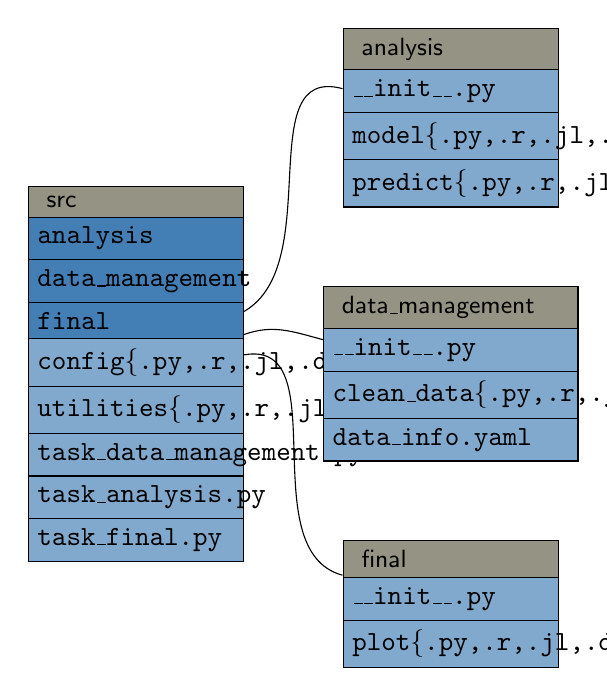
\begin{tikzpicture}[node distance=1cm, auto]

        \node (3) [
            rectangle split,
            rectangle split parts=9,
            rectangle split part fill={
                gray,
                blue!75,
                blue!75,
                blue!75,
                blue!50,
                blue!50,
                blue!50,
                blue!50,
                blue!50,
            },
            draw,
            text width=2.50cm
        ]
        {
            \nodepart{one}
                \begin{small}
                    src
                \end{small}
            \nodepart{two}
                \texttt{analysis}
            \nodepart{three}
                \texttt{data\_management}
            \nodepart{four}
                \texttt{final}
            \nodepart{five}
                \texttt{config\{.py,.r,.jl,.do\}}
            \nodepart{six}
                \texttt{utilities\{.py,.r,.jl,.do\}}
            \nodepart{seven}
                \texttt{task\_data\_management.py}
            \nodepart{eight}
                \texttt{task\_analysis.py}
            \nodepart{nine}
                \texttt{task\_final.py}
        };

        \node (4) [
            rectangle split,
            rectangle split parts=4,
            rectangle split part fill={
                gray,
                blue!50,
                blue!50,
                blue!50,
            },
            draw,
            text width=3.0cm,
            right=of 3
        ]
        {
            \nodepart{one}
                \begin{small}
                    data\_management
                \end{small}
            \nodepart{two}
                \texttt{\_\_init\_\_.py}
            \nodepart{three}
                \texttt{clean\_data\{.py,.r,.jl,.do\}}
            \nodepart{four}
                \texttt{data\_info.yaml}
        };

        \node (5) [
            rectangle split,
            rectangle split parts=4,
            rectangle split part fill={
                gray,
                blue!50,
                blue!50,
                blue!50,
            },
            draw,
            text width=2.5cm,
            above=of 4
        ]
        {
            \nodepart{one}
                \begin{small}
                    analysis
                \end{small}
            \nodepart{two}
                \texttt{\_\_init\_\_.py}
            \nodepart{three}
                \texttt{model\{.py,.r,.jl,.do\}}
            \nodepart{four}
                \texttt{predict\{.py,.r,.jl,.do\}}
        };

        \node (6) [
            rectangle split,
            rectangle split parts=3,
            rectangle split part fill={
                gray,
                blue!50,
                blue!50,
            },
            draw,
            text width=2.5cm,
            below=of 4
        ]
        {
            \nodepart{one}
                \begin{small}
                    final
                \end{small}
            \nodepart{two}
                \texttt{\_\_init\_\_.py}
            \nodepart{three}
                \texttt{plot\{.py,.r,.jl,.do\}}
        };

        \draw[-, out=20, in=165] (3) to (4);
        \draw[-, out=30, in=165] (3) to (5);
        \draw[-, out=10, in=165] (3) to (6);
    \end{tikzpicture}}
\end{tiny}

\end{document}
